\section{Edward Francis O'Brien Jr.}\label{per:Edward4OBrien3}

\begin{figure}[htbp]
	\centering
	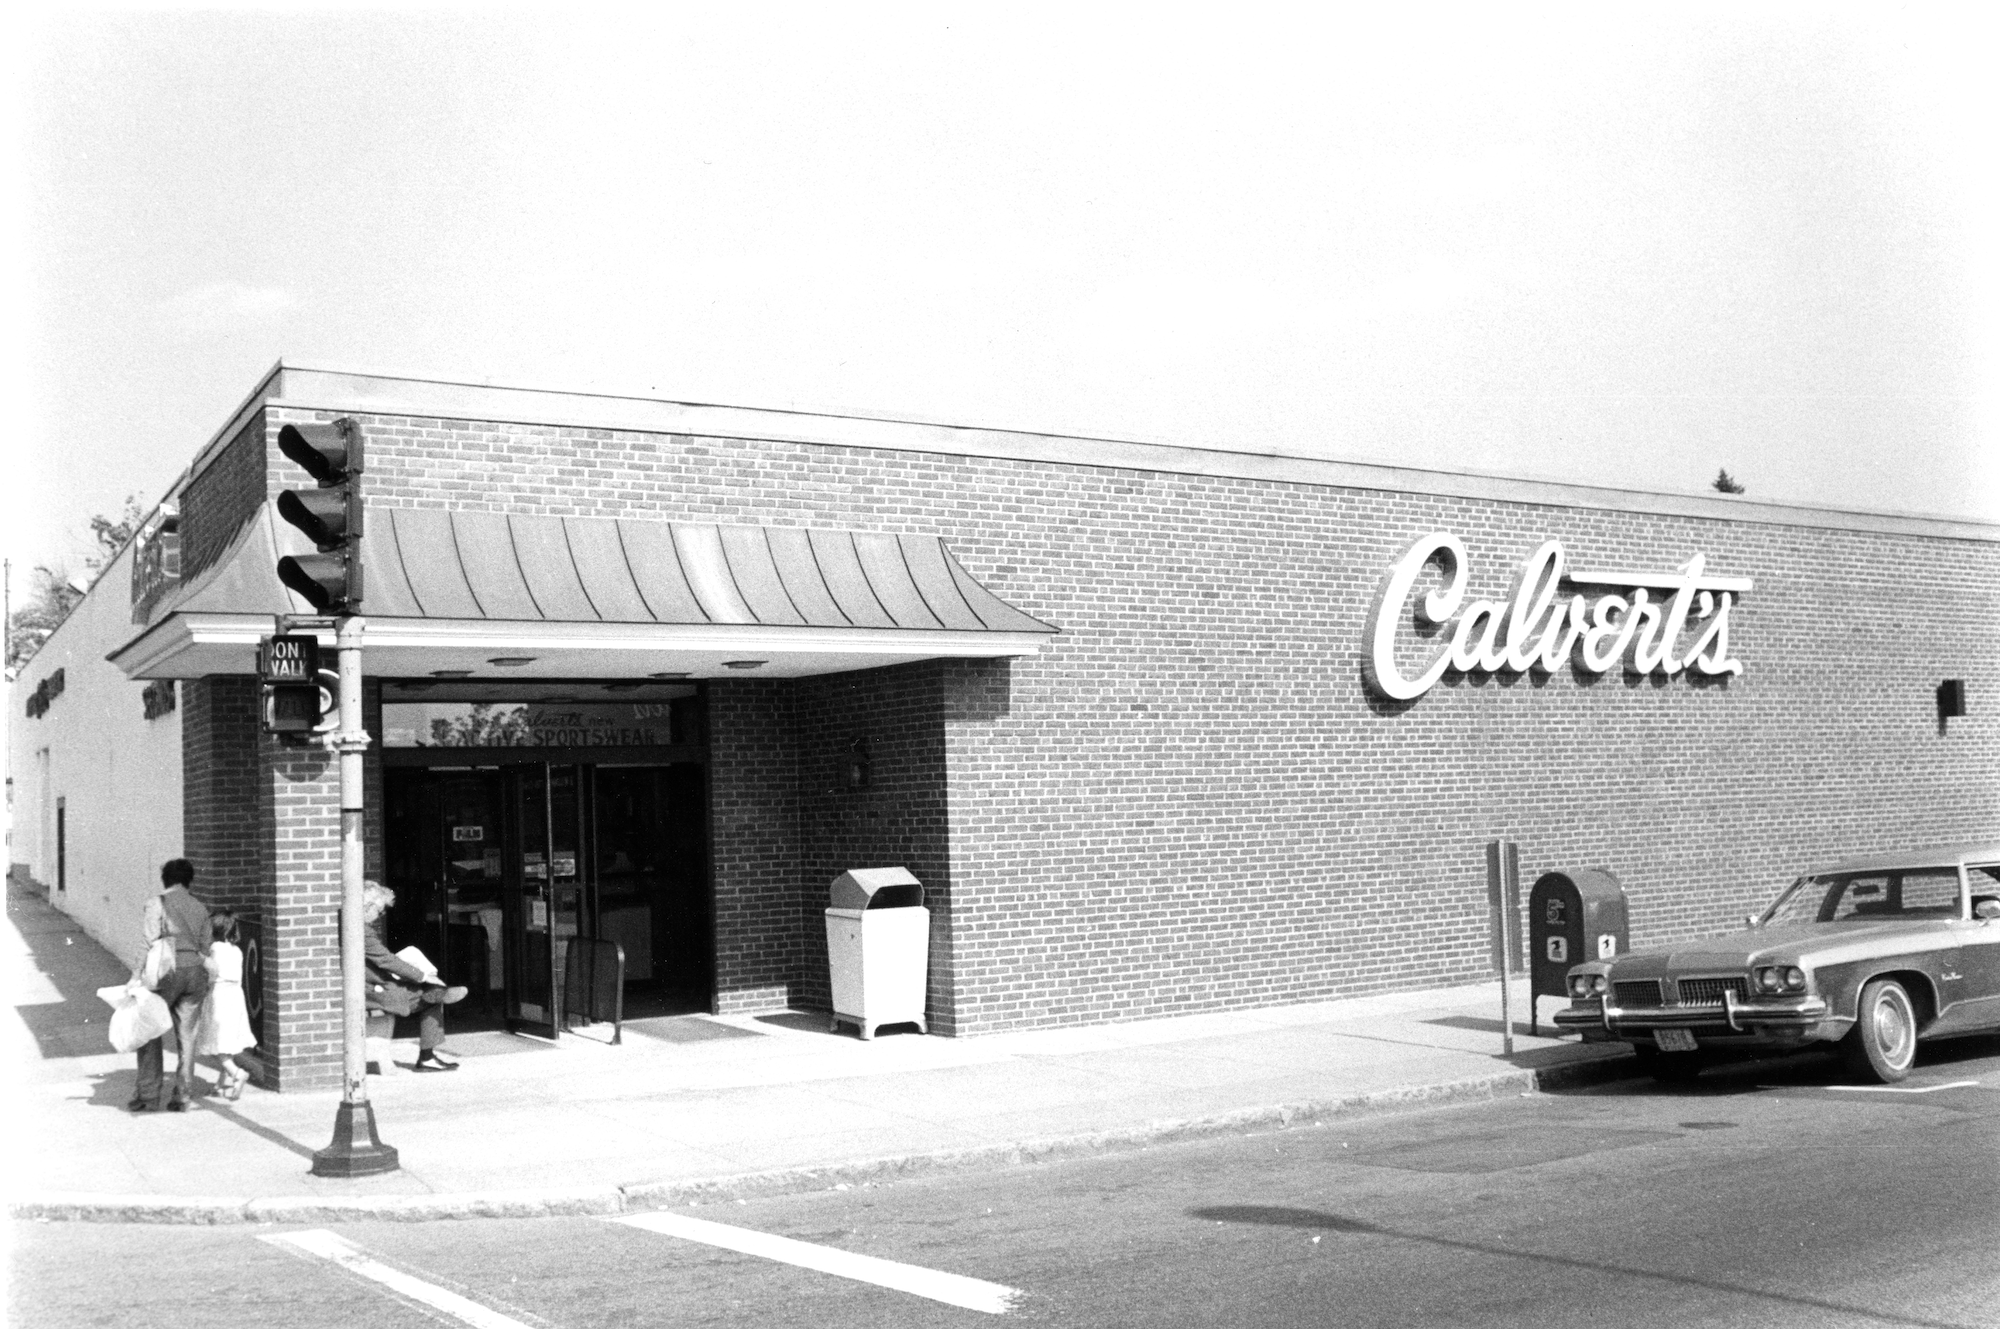
\includegraphics[width=\textwidth]{calverts}
	\caption{Calvert's Clothing Store\index{Calvert's Department Store}, June 1979}
	\label{fig:Calverts}
\end{figure}

\MainPerson{Edward Francis\textsuperscript{4} O'Brien Jr.}\index{O'Brien!Edward Francis\textsuperscript{4} Jr. (1916--1985)|bb} (\Lineage{3}{Edward}, \Lineage{2}{Michael}, \Lineage{1}{William}) was born in Boston, Suffolk County, Massachusetts,\index{Massachusetts!Boston} on 17 September 1916.\cite{Edward4OBrien3Birth} He died suddenly in Needham, Norfolk County, Massachusetts,\index{Massachusetts!Needham} on 12 December 1985.\cite{Edward4OBrien3Death,Edward4OBrien3Obit:1} He married, in Milton, Norfolk County, Massachusetts,\index{Massachusetts!Milton} in 1946, \MainPerson{Mary Anne Metivier}.\index{Metivier!Mary Anne}\index{O'Brien!Mary Anne (Metivier)}\cite{Edward4OBrien3Marriage} She was born in Milton\index{Massachusetts!Milton} on 25 November 1917 to Wilfrid Metivier\index{Metivier!Wilfred} and Helen (Day) Metivier.\index{Metivier!Helen (Day)}\index{Day!Helen}\cite{MaryMetivierBirth} She died in Needham\index{Massachusetts!Needham} on 29 August 1999.\cite{MaryMetivierDeath}

Edward\index{O'Brien!Edward Francis\textsuperscript{4}, Jr. (1916--1985)} was the general manager of Calvert's Department Store\index{Calvert's Department Store} in Needham,\index{Massachusetts!Needham} where he worked for 38 years. He was an Army\index{Army} captain in World War II\index{World War II} and the Korean War.\index{Korean War} Edward also served as vice president and director of the Needham Cooperative Bank,\index{Needham Cooperative Bank} a member of the Needham Board of Appeals, and a Needham Town Meeting member.\cite{Edward4OBrien3Obit:2}

\begin{KidsIntro}
	Children of Edward F.\textsuperscript{4} O'Brien Jr.\index{O'Brien!Edward Francis\textsuperscript{4}, Jr. (1916--1985)} and Mary A.\ (Metivier) O'Brien:\index{Metivier!Mary Anne}\index{O'Brien!Mary Anne (Metivier)}
\end{KidsIntro}

\begin{Kids}
	\KidNum{}{$\bullet$}\KidName{Clare\textsuperscript{5} O'Brien}\index{O'Brien!Clare\textsuperscript{5}}
	
	\KidNum{}{$\bullet$}\KidName{Julie O'Brien}\index{O'Brien!Julie\textsuperscript{5}}
	
	\KidNum{}{$\bullet$}\KidName{Ted O'Brien}\index{O'Brien!Ted\textsuperscript{5}}
	
	\KidNum{}{$\bullet$}\KidName{Ellen O'Brien}\index{O'Brien!Ellen\textsuperscript{5}}
\end{Kids}
